
% Default to the notebook output style

    


% Inherit from the specified cell style.




    
\documentclass[11pt]{article}

    
    
    \usepackage[T1]{fontenc}
    % Nicer default font (+ math font) than Computer Modern for most use cases
    \usepackage{mathpazo}

    % Basic figure setup, for now with no caption control since it's done
    % automatically by Pandoc (which extracts ![](path) syntax from Markdown).
    \usepackage{graphicx}
    % We will generate all images so they have a width \maxwidth. This means
    % that they will get their normal width if they fit onto the page, but
    % are scaled down if they would overflow the margins.
    \makeatletter
    \def\maxwidth{\ifdim\Gin@nat@width>\linewidth\linewidth
    \else\Gin@nat@width\fi}
    \makeatother
    \let\Oldincludegraphics\includegraphics
    % Set max figure width to be 80% of text width, for now hardcoded.
    \renewcommand{\includegraphics}[1]{\Oldincludegraphics[width=.8\maxwidth]{#1}}
    % Ensure that by default, figures have no caption (until we provide a
    % proper Figure object with a Caption API and a way to capture that
    % in the conversion process - todo).
    \usepackage{caption}
    \DeclareCaptionLabelFormat{nolabel}{}
    \captionsetup{labelformat=nolabel}

    \usepackage{adjustbox} % Used to constrain images to a maximum size 
    \usepackage{xcolor} % Allow colors to be defined
    \usepackage{enumerate} % Needed for markdown enumerations to work
    \usepackage{geometry} % Used to adjust the document margins
    \usepackage{amsmath} % Equations
    \usepackage{amssymb} % Equations
    \usepackage{textcomp} % defines textquotesingle
    % Hack from http://tex.stackexchange.com/a/47451/13684:
    \AtBeginDocument{%
        \def\PYZsq{\textquotesingle}% Upright quotes in Pygmentized code
    }
    \usepackage{upquote} % Upright quotes for verbatim code
    \usepackage{eurosym} % defines \euro
    \usepackage[mathletters]{ucs} % Extended unicode (utf-8) support
    \usepackage[utf8x]{inputenc} % Allow utf-8 characters in the tex document
    \usepackage{fancyvrb} % verbatim replacement that allows latex
    \usepackage{grffile} % extends the file name processing of package graphics 
                         % to support a larger range 
    % The hyperref package gives us a pdf with properly built
    % internal navigation ('pdf bookmarks' for the table of contents,
    % internal cross-reference links, web links for URLs, etc.)
    \usepackage{hyperref}
    \usepackage{longtable} % longtable support required by pandoc >1.10
    \usepackage{booktabs}  % table support for pandoc > 1.12.2
    \usepackage[inline]{enumitem} % IRkernel/repr support (it uses the enumerate* environment)
    \usepackage[normalem]{ulem} % ulem is needed to support strikethroughs (\sout)
                                % normalem makes italics be italics, not underlines
    

    
    
    % Colors for the hyperref package
    \definecolor{urlcolor}{rgb}{0,.145,.698}
    \definecolor{linkcolor}{rgb}{.71,0.21,0.01}
    \definecolor{citecolor}{rgb}{.12,.54,.11}

    % ANSI colors
    \definecolor{ansi-black}{HTML}{3E424D}
    \definecolor{ansi-black-intense}{HTML}{282C36}
    \definecolor{ansi-red}{HTML}{E75C58}
    \definecolor{ansi-red-intense}{HTML}{B22B31}
    \definecolor{ansi-green}{HTML}{00A250}
    \definecolor{ansi-green-intense}{HTML}{007427}
    \definecolor{ansi-yellow}{HTML}{DDB62B}
    \definecolor{ansi-yellow-intense}{HTML}{B27D12}
    \definecolor{ansi-blue}{HTML}{208FFB}
    \definecolor{ansi-blue-intense}{HTML}{0065CA}
    \definecolor{ansi-magenta}{HTML}{D160C4}
    \definecolor{ansi-magenta-intense}{HTML}{A03196}
    \definecolor{ansi-cyan}{HTML}{60C6C8}
    \definecolor{ansi-cyan-intense}{HTML}{258F8F}
    \definecolor{ansi-white}{HTML}{C5C1B4}
    \definecolor{ansi-white-intense}{HTML}{A1A6B2}

    % commands and environments needed by pandoc snippets
    % extracted from the output of `pandoc -s`
    \providecommand{\tightlist}{%
      \setlength{\itemsep}{0pt}\setlength{\parskip}{0pt}}
    \DefineVerbatimEnvironment{Highlighting}{Verbatim}{commandchars=\\\{\}}
    % Add ',fontsize=\small' for more characters per line
    \newenvironment{Shaded}{}{}
    \newcommand{\KeywordTok}[1]{\textcolor[rgb]{0.00,0.44,0.13}{\textbf{{#1}}}}
    \newcommand{\DataTypeTok}[1]{\textcolor[rgb]{0.56,0.13,0.00}{{#1}}}
    \newcommand{\DecValTok}[1]{\textcolor[rgb]{0.25,0.63,0.44}{{#1}}}
    \newcommand{\BaseNTok}[1]{\textcolor[rgb]{0.25,0.63,0.44}{{#1}}}
    \newcommand{\FloatTok}[1]{\textcolor[rgb]{0.25,0.63,0.44}{{#1}}}
    \newcommand{\CharTok}[1]{\textcolor[rgb]{0.25,0.44,0.63}{{#1}}}
    \newcommand{\StringTok}[1]{\textcolor[rgb]{0.25,0.44,0.63}{{#1}}}
    \newcommand{\CommentTok}[1]{\textcolor[rgb]{0.38,0.63,0.69}{\textit{{#1}}}}
    \newcommand{\OtherTok}[1]{\textcolor[rgb]{0.00,0.44,0.13}{{#1}}}
    \newcommand{\AlertTok}[1]{\textcolor[rgb]{1.00,0.00,0.00}{\textbf{{#1}}}}
    \newcommand{\FunctionTok}[1]{\textcolor[rgb]{0.02,0.16,0.49}{{#1}}}
    \newcommand{\RegionMarkerTok}[1]{{#1}}
    \newcommand{\ErrorTok}[1]{\textcolor[rgb]{1.00,0.00,0.00}{\textbf{{#1}}}}
    \newcommand{\NormalTok}[1]{{#1}}
    
    % Additional commands for more recent versions of Pandoc
    \newcommand{\ConstantTok}[1]{\textcolor[rgb]{0.53,0.00,0.00}{{#1}}}
    \newcommand{\SpecialCharTok}[1]{\textcolor[rgb]{0.25,0.44,0.63}{{#1}}}
    \newcommand{\VerbatimStringTok}[1]{\textcolor[rgb]{0.25,0.44,0.63}{{#1}}}
    \newcommand{\SpecialStringTok}[1]{\textcolor[rgb]{0.73,0.40,0.53}{{#1}}}
    \newcommand{\ImportTok}[1]{{#1}}
    \newcommand{\DocumentationTok}[1]{\textcolor[rgb]{0.73,0.13,0.13}{\textit{{#1}}}}
    \newcommand{\AnnotationTok}[1]{\textcolor[rgb]{0.38,0.63,0.69}{\textbf{\textit{{#1}}}}}
    \newcommand{\CommentVarTok}[1]{\textcolor[rgb]{0.38,0.63,0.69}{\textbf{\textit{{#1}}}}}
    \newcommand{\VariableTok}[1]{\textcolor[rgb]{0.10,0.09,0.49}{{#1}}}
    \newcommand{\ControlFlowTok}[1]{\textcolor[rgb]{0.00,0.44,0.13}{\textbf{{#1}}}}
    \newcommand{\OperatorTok}[1]{\textcolor[rgb]{0.40,0.40,0.40}{{#1}}}
    \newcommand{\BuiltInTok}[1]{{#1}}
    \newcommand{\ExtensionTok}[1]{{#1}}
    \newcommand{\PreprocessorTok}[1]{\textcolor[rgb]{0.74,0.48,0.00}{{#1}}}
    \newcommand{\AttributeTok}[1]{\textcolor[rgb]{0.49,0.56,0.16}{{#1}}}
    \newcommand{\InformationTok}[1]{\textcolor[rgb]{0.38,0.63,0.69}{\textbf{\textit{{#1}}}}}
    \newcommand{\WarningTok}[1]{\textcolor[rgb]{0.38,0.63,0.69}{\textbf{\textit{{#1}}}}}
    
    
    % Define a nice break command that doesn't care if a line doesn't already
    % exist.
    \def\br{\hspace*{\fill} \\* }
    % Math Jax compatability definitions
    \def\gt{>}
    \def\lt{<}
    % Document parameters
    \title{GM-10 Experiments}
    
    
    

    % Pygments definitions
    
\makeatletter
\def\PY@reset{\let\PY@it=\relax \let\PY@bf=\relax%
    \let\PY@ul=\relax \let\PY@tc=\relax%
    \let\PY@bc=\relax \let\PY@ff=\relax}
\def\PY@tok#1{\csname PY@tok@#1\endcsname}
\def\PY@toks#1+{\ifx\relax#1\empty\else%
    \PY@tok{#1}\expandafter\PY@toks\fi}
\def\PY@do#1{\PY@bc{\PY@tc{\PY@ul{%
    \PY@it{\PY@bf{\PY@ff{#1}}}}}}}
\def\PY#1#2{\PY@reset\PY@toks#1+\relax+\PY@do{#2}}

\expandafter\def\csname PY@tok@il\endcsname{\def\PY@tc##1{\textcolor[rgb]{0.40,0.40,0.40}{##1}}}
\expandafter\def\csname PY@tok@kc\endcsname{\let\PY@bf=\textbf\def\PY@tc##1{\textcolor[rgb]{0.00,0.50,0.00}{##1}}}
\expandafter\def\csname PY@tok@nd\endcsname{\def\PY@tc##1{\textcolor[rgb]{0.67,0.13,1.00}{##1}}}
\expandafter\def\csname PY@tok@sr\endcsname{\def\PY@tc##1{\textcolor[rgb]{0.73,0.40,0.53}{##1}}}
\expandafter\def\csname PY@tok@dl\endcsname{\def\PY@tc##1{\textcolor[rgb]{0.73,0.13,0.13}{##1}}}
\expandafter\def\csname PY@tok@gp\endcsname{\let\PY@bf=\textbf\def\PY@tc##1{\textcolor[rgb]{0.00,0.00,0.50}{##1}}}
\expandafter\def\csname PY@tok@nb\endcsname{\def\PY@tc##1{\textcolor[rgb]{0.00,0.50,0.00}{##1}}}
\expandafter\def\csname PY@tok@kt\endcsname{\def\PY@tc##1{\textcolor[rgb]{0.69,0.00,0.25}{##1}}}
\expandafter\def\csname PY@tok@mi\endcsname{\def\PY@tc##1{\textcolor[rgb]{0.40,0.40,0.40}{##1}}}
\expandafter\def\csname PY@tok@mf\endcsname{\def\PY@tc##1{\textcolor[rgb]{0.40,0.40,0.40}{##1}}}
\expandafter\def\csname PY@tok@k\endcsname{\let\PY@bf=\textbf\def\PY@tc##1{\textcolor[rgb]{0.00,0.50,0.00}{##1}}}
\expandafter\def\csname PY@tok@na\endcsname{\def\PY@tc##1{\textcolor[rgb]{0.49,0.56,0.16}{##1}}}
\expandafter\def\csname PY@tok@m\endcsname{\def\PY@tc##1{\textcolor[rgb]{0.40,0.40,0.40}{##1}}}
\expandafter\def\csname PY@tok@ss\endcsname{\def\PY@tc##1{\textcolor[rgb]{0.10,0.09,0.49}{##1}}}
\expandafter\def\csname PY@tok@err\endcsname{\def\PY@bc##1{\setlength{\fboxsep}{0pt}\fcolorbox[rgb]{1.00,0.00,0.00}{1,1,1}{\strut ##1}}}
\expandafter\def\csname PY@tok@no\endcsname{\def\PY@tc##1{\textcolor[rgb]{0.53,0.00,0.00}{##1}}}
\expandafter\def\csname PY@tok@vc\endcsname{\def\PY@tc##1{\textcolor[rgb]{0.10,0.09,0.49}{##1}}}
\expandafter\def\csname PY@tok@mh\endcsname{\def\PY@tc##1{\textcolor[rgb]{0.40,0.40,0.40}{##1}}}
\expandafter\def\csname PY@tok@si\endcsname{\let\PY@bf=\textbf\def\PY@tc##1{\textcolor[rgb]{0.73,0.40,0.53}{##1}}}
\expandafter\def\csname PY@tok@gs\endcsname{\let\PY@bf=\textbf}
\expandafter\def\csname PY@tok@o\endcsname{\def\PY@tc##1{\textcolor[rgb]{0.40,0.40,0.40}{##1}}}
\expandafter\def\csname PY@tok@kp\endcsname{\def\PY@tc##1{\textcolor[rgb]{0.00,0.50,0.00}{##1}}}
\expandafter\def\csname PY@tok@gu\endcsname{\let\PY@bf=\textbf\def\PY@tc##1{\textcolor[rgb]{0.50,0.00,0.50}{##1}}}
\expandafter\def\csname PY@tok@nc\endcsname{\let\PY@bf=\textbf\def\PY@tc##1{\textcolor[rgb]{0.00,0.00,1.00}{##1}}}
\expandafter\def\csname PY@tok@gh\endcsname{\let\PY@bf=\textbf\def\PY@tc##1{\textcolor[rgb]{0.00,0.00,0.50}{##1}}}
\expandafter\def\csname PY@tok@sd\endcsname{\let\PY@it=\textit\def\PY@tc##1{\textcolor[rgb]{0.73,0.13,0.13}{##1}}}
\expandafter\def\csname PY@tok@w\endcsname{\def\PY@tc##1{\textcolor[rgb]{0.73,0.73,0.73}{##1}}}
\expandafter\def\csname PY@tok@kr\endcsname{\let\PY@bf=\textbf\def\PY@tc##1{\textcolor[rgb]{0.00,0.50,0.00}{##1}}}
\expandafter\def\csname PY@tok@fm\endcsname{\def\PY@tc##1{\textcolor[rgb]{0.00,0.00,1.00}{##1}}}
\expandafter\def\csname PY@tok@sb\endcsname{\def\PY@tc##1{\textcolor[rgb]{0.73,0.13,0.13}{##1}}}
\expandafter\def\csname PY@tok@mo\endcsname{\def\PY@tc##1{\textcolor[rgb]{0.40,0.40,0.40}{##1}}}
\expandafter\def\csname PY@tok@nl\endcsname{\def\PY@tc##1{\textcolor[rgb]{0.63,0.63,0.00}{##1}}}
\expandafter\def\csname PY@tok@sc\endcsname{\def\PY@tc##1{\textcolor[rgb]{0.73,0.13,0.13}{##1}}}
\expandafter\def\csname PY@tok@mb\endcsname{\def\PY@tc##1{\textcolor[rgb]{0.40,0.40,0.40}{##1}}}
\expandafter\def\csname PY@tok@cp\endcsname{\def\PY@tc##1{\textcolor[rgb]{0.74,0.48,0.00}{##1}}}
\expandafter\def\csname PY@tok@cpf\endcsname{\let\PY@it=\textit\def\PY@tc##1{\textcolor[rgb]{0.25,0.50,0.50}{##1}}}
\expandafter\def\csname PY@tok@ni\endcsname{\let\PY@bf=\textbf\def\PY@tc##1{\textcolor[rgb]{0.60,0.60,0.60}{##1}}}
\expandafter\def\csname PY@tok@sx\endcsname{\def\PY@tc##1{\textcolor[rgb]{0.00,0.50,0.00}{##1}}}
\expandafter\def\csname PY@tok@cm\endcsname{\let\PY@it=\textit\def\PY@tc##1{\textcolor[rgb]{0.25,0.50,0.50}{##1}}}
\expandafter\def\csname PY@tok@ge\endcsname{\let\PY@it=\textit}
\expandafter\def\csname PY@tok@kd\endcsname{\let\PY@bf=\textbf\def\PY@tc##1{\textcolor[rgb]{0.00,0.50,0.00}{##1}}}
\expandafter\def\csname PY@tok@c1\endcsname{\let\PY@it=\textit\def\PY@tc##1{\textcolor[rgb]{0.25,0.50,0.50}{##1}}}
\expandafter\def\csname PY@tok@cs\endcsname{\let\PY@it=\textit\def\PY@tc##1{\textcolor[rgb]{0.25,0.50,0.50}{##1}}}
\expandafter\def\csname PY@tok@sa\endcsname{\def\PY@tc##1{\textcolor[rgb]{0.73,0.13,0.13}{##1}}}
\expandafter\def\csname PY@tok@nv\endcsname{\def\PY@tc##1{\textcolor[rgb]{0.10,0.09,0.49}{##1}}}
\expandafter\def\csname PY@tok@vg\endcsname{\def\PY@tc##1{\textcolor[rgb]{0.10,0.09,0.49}{##1}}}
\expandafter\def\csname PY@tok@bp\endcsname{\def\PY@tc##1{\textcolor[rgb]{0.00,0.50,0.00}{##1}}}
\expandafter\def\csname PY@tok@kn\endcsname{\let\PY@bf=\textbf\def\PY@tc##1{\textcolor[rgb]{0.00,0.50,0.00}{##1}}}
\expandafter\def\csname PY@tok@ne\endcsname{\let\PY@bf=\textbf\def\PY@tc##1{\textcolor[rgb]{0.82,0.25,0.23}{##1}}}
\expandafter\def\csname PY@tok@c\endcsname{\let\PY@it=\textit\def\PY@tc##1{\textcolor[rgb]{0.25,0.50,0.50}{##1}}}
\expandafter\def\csname PY@tok@nt\endcsname{\let\PY@bf=\textbf\def\PY@tc##1{\textcolor[rgb]{0.00,0.50,0.00}{##1}}}
\expandafter\def\csname PY@tok@sh\endcsname{\def\PY@tc##1{\textcolor[rgb]{0.73,0.13,0.13}{##1}}}
\expandafter\def\csname PY@tok@ow\endcsname{\let\PY@bf=\textbf\def\PY@tc##1{\textcolor[rgb]{0.67,0.13,1.00}{##1}}}
\expandafter\def\csname PY@tok@s\endcsname{\def\PY@tc##1{\textcolor[rgb]{0.73,0.13,0.13}{##1}}}
\expandafter\def\csname PY@tok@s1\endcsname{\def\PY@tc##1{\textcolor[rgb]{0.73,0.13,0.13}{##1}}}
\expandafter\def\csname PY@tok@vm\endcsname{\def\PY@tc##1{\textcolor[rgb]{0.10,0.09,0.49}{##1}}}
\expandafter\def\csname PY@tok@gt\endcsname{\def\PY@tc##1{\textcolor[rgb]{0.00,0.27,0.87}{##1}}}
\expandafter\def\csname PY@tok@s2\endcsname{\def\PY@tc##1{\textcolor[rgb]{0.73,0.13,0.13}{##1}}}
\expandafter\def\csname PY@tok@nn\endcsname{\let\PY@bf=\textbf\def\PY@tc##1{\textcolor[rgb]{0.00,0.00,1.00}{##1}}}
\expandafter\def\csname PY@tok@ch\endcsname{\let\PY@it=\textit\def\PY@tc##1{\textcolor[rgb]{0.25,0.50,0.50}{##1}}}
\expandafter\def\csname PY@tok@vi\endcsname{\def\PY@tc##1{\textcolor[rgb]{0.10,0.09,0.49}{##1}}}
\expandafter\def\csname PY@tok@gd\endcsname{\def\PY@tc##1{\textcolor[rgb]{0.63,0.00,0.00}{##1}}}
\expandafter\def\csname PY@tok@se\endcsname{\let\PY@bf=\textbf\def\PY@tc##1{\textcolor[rgb]{0.73,0.40,0.13}{##1}}}
\expandafter\def\csname PY@tok@go\endcsname{\def\PY@tc##1{\textcolor[rgb]{0.53,0.53,0.53}{##1}}}
\expandafter\def\csname PY@tok@gr\endcsname{\def\PY@tc##1{\textcolor[rgb]{1.00,0.00,0.00}{##1}}}
\expandafter\def\csname PY@tok@gi\endcsname{\def\PY@tc##1{\textcolor[rgb]{0.00,0.63,0.00}{##1}}}
\expandafter\def\csname PY@tok@nf\endcsname{\def\PY@tc##1{\textcolor[rgb]{0.00,0.00,1.00}{##1}}}

\def\PYZbs{\char`\\}
\def\PYZus{\char`\_}
\def\PYZob{\char`\{}
\def\PYZcb{\char`\}}
\def\PYZca{\char`\^}
\def\PYZam{\char`\&}
\def\PYZlt{\char`\<}
\def\PYZgt{\char`\>}
\def\PYZsh{\char`\#}
\def\PYZpc{\char`\%}
\def\PYZdl{\char`\$}
\def\PYZhy{\char`\-}
\def\PYZsq{\char`\'}
\def\PYZdq{\char`\"}
\def\PYZti{\char`\~}
% for compatibility with earlier versions
\def\PYZat{@}
\def\PYZlb{[}
\def\PYZrb{]}
\makeatother


    % Exact colors from NB
    \definecolor{incolor}{rgb}{0.0, 0.0, 0.5}
    \definecolor{outcolor}{rgb}{0.545, 0.0, 0.0}



    
    % Prevent overflowing lines due to hard-to-break entities
    \sloppy 
    % Setup hyperref package
    \hypersetup{
      breaklinks=true,  % so long urls are correctly broken across lines
      colorlinks=true,
      urlcolor=urlcolor,
      linkcolor=linkcolor,
      citecolor=citecolor,
      }
    % Slightly bigger margins than the latex defaults
    
    \geometry{verbose,tmargin=1in,bmargin=1in,lmargin=1in,rmargin=1in}
    
    

    \begin{document}
    
    
    \maketitle
    
    

    
    \section{Is my Smoke Detector
Radioactive?}\label{is-my-smoke-detector-radioactive}

\subsubsection{Data Analysis from Python and a GM-10 Device in Mountain
View,
CA}\label{data-analysis-from-python-and-a-gm-10-device-in-mountain-view-ca}

Thanks to Keith E. Fleming for loaning me the GM-10

\begin{figure}
\centering

\includegraphics{./corona.jpeg}
\caption{corona}
\end{figure}

\begin{center}\rule{0.5\linewidth}{\linethickness}\end{center}

    In this paper we will play around with some overly simple science and
stats related to radiation sources as they are captured from a GM-10
Geiger Counter Radiation Detector in Mountain View, CA in late Jan /
early Feb 2018.

\subsubsection{About the GM-10}\label{about-the-gm-10}

The GM-10 contains a geiger mueller tube, capable of detecting alpha,
beta, and gamma / x-ray radiation. Each time a radiation particle enters
the sensing window, it is detected, and the software on the attached
computer is informed of this event.

By adding up the number of detections per minute, the Counts Per Minute
(CPM) is calculated and displayed. This number is a relative indicator
of the amount of radiation present.

See http://www.blackcatsystems.com/GM/products/GM10GeigerCounter.html

\subsubsection{A Note on Normal Background
Radiation}\label{a-note-on-normal-background-radiation}

Background radiation is the ionizing radiation present in the
environment. Background radiation originates from a variety of sources,
both natural and artificial. Sources include cosmic radiation, and
environmental radioactivity from such as naturally occurring radioactive
materials including radon and radium, and fallout from nuclear weapons
testing and nuclear accidents.

\subsubsection{A Note on Mountain View,
CA}\label{a-note-on-mountain-view-ca}

Mountain View is a city located in Santa Clara County, California,
United States, named for its views of the Santa Cruz Mountains. From its
origins as a stagecoach stop, it grew to a large suburb with a
pedestrian-friendly downtown and a population of 74,066. The city
borders Palo Alto and the San Francisco Bay to the north, Los Altos to
the south, and Moffett Federal Airfield and Sunnyvale to the east.

Elevation 105 ft (32 m)

    \subsection{\#\# On to the code...}\label{on-to-the-code...}

    \subsubsection{Loading the data}\label{loading-the-data}

Over a period of several weeks I ran a series of tests using the GM-10.
The device can be set to store its readings to a file. The readings are
in a flat file with the format or "date\_time", "reading in CM."

    \begin{Verbatim}[commandchars=\\\{\}]
{\color{incolor}In [{\color{incolor}8}]:} \PY{k+kn}{import} \PY{n+nn}{pandas} \PY{k}{as} \PY{n+nn}{pd}
        
        \PY{c+c1}{\PYZsh{}\PYZsh{}\PYZsh{}\PYZsh{}\PYZsh{}\PYZsh{}\PYZsh{}\PYZsh{}\PYZsh{}\PYZsh{}\PYZsh{}\PYZsh{}\PYZsh{}\PYZsh{}\PYZsh{}\PYZsh{}\PYZsh{}\PYZsh{}\PYZsh{}\PYZsh{}\PYZsh{}\PYZsh{}\PYZsh{}\PYZsh{}\PYZsh{}\PYZsh{}\PYZsh{}\PYZsh{}\PYZsh{}\PYZsh{}\PYZsh{}\PYZsh{}\PYZsh{}\PYZsh{}\PYZsh{}\PYZsh{}\PYZsh{}\PYZsh{}\PYZsh{}\PYZsh{}\PYZsh{}\PYZsh{}\PYZsh{}\PYZsh{}\PYZsh{}\PYZsh{}\PYZsh{}\PYZsh{}\PYZsh{}\PYZsh{}\PYZsh{}\PYZsh{}\PYZsh{}\PYZsh{}\PYZsh{}\PYZsh{}\PYZsh{}\PYZsh{}\PYZsh{}\PYZsh{}\PYZsh{}\PYZsh{}\PYZsh{}\PYZsh{}\PYZsh{}\PYZsh{}\PYZsh{}\PYZsh{}\PYZsh{}\PYZsh{}\PYZsh{}\PYZsh{}\PYZsh{}\PYZsh{}\PYZsh{}\PYZsh{}\PYZsh{}\PYZsh{}\PYZsh{}\PYZsh{}\PYZsh{}\PYZsh{}\PYZsh{}\PYZsh{}\PYZsh{}\PYZsh{}\PYZsh{}\PYZsh{}\PYZsh{}\PYZsh{}}
        \PY{c+c1}{\PYZsh{} Baselines}
        \PY{c+c1}{\PYZsh{}\PYZsh{}\PYZsh{}\PYZsh{}\PYZsh{}\PYZsh{}\PYZsh{}\PYZsh{}\PYZsh{}\PYZsh{}\PYZsh{}\PYZsh{}\PYZsh{}\PYZsh{}\PYZsh{}\PYZsh{}\PYZsh{}\PYZsh{}\PYZsh{}\PYZsh{}\PYZsh{}\PYZsh{}\PYZsh{}\PYZsh{}\PYZsh{}\PYZsh{}\PYZsh{}\PYZsh{}\PYZsh{}\PYZsh{}\PYZsh{}\PYZsh{}\PYZsh{}\PYZsh{}\PYZsh{}\PYZsh{}\PYZsh{}\PYZsh{}\PYZsh{}\PYZsh{}\PYZsh{}\PYZsh{}\PYZsh{}\PYZsh{}\PYZsh{}\PYZsh{}\PYZsh{}\PYZsh{}\PYZsh{}\PYZsh{}\PYZsh{}\PYZsh{}\PYZsh{}\PYZsh{}\PYZsh{}\PYZsh{}\PYZsh{}\PYZsh{}\PYZsh{}\PYZsh{}\PYZsh{}\PYZsh{}\PYZsh{}\PYZsh{}\PYZsh{}\PYZsh{}\PYZsh{}\PYZsh{}\PYZsh{}\PYZsh{}\PYZsh{}\PYZsh{}\PYZsh{}\PYZsh{}\PYZsh{}\PYZsh{}\PYZsh{}\PYZsh{}\PYZsh{}\PYZsh{}\PYZsh{}\PYZsh{}\PYZsh{}\PYZsh{}\PYZsh{}\PYZsh{}\PYZsh{}\PYZsh{}\PYZsh{}\PYZsh{}}
        
        \PY{n+nb}{print}\PY{p}{(}\PY{l+s+s2}{\PYZdq{}}\PY{l+s+s2}{Loading the data... The sizes reported are (observations, attributes).}\PY{l+s+s2}{\PYZdq{}}\PY{p}{)}
        \PY{c+c1}{\PYZsh{} rad\PYZus{}recording\PYZhy{}1\PYZhy{}16\PYZhy{}18 \PYZhy{} orginal baseline}
        \PY{n}{rad\PYZus{}recording01162018} \PY{o}{=} \PY{n}{pd}\PY{o}{.}\PY{n}{read\PYZus{}csv}\PY{p}{(}\PY{l+s+s1}{\PYZsq{}}\PY{l+s+s1}{./data/rad\PYZus{}recording\PYZhy{}1\PYZhy{}16\PYZhy{}18}\PY{l+s+s1}{\PYZsq{}}\PY{p}{,} \PY{n}{header}\PY{o}{=}\PY{k+kc}{None} \PY{p}{)}
        \PY{n}{rad\PYZus{}recording01162018}\PY{o}{.}\PY{n}{columns} \PY{o}{=} \PY{p}{[}\PY{l+s+s1}{\PYZsq{}}\PY{l+s+s1}{DateAndTime}\PY{l+s+s1}{\PYZsq{}}\PY{p}{,} \PY{l+s+s1}{\PYZsq{}}\PY{l+s+s1}{Reading}\PY{l+s+s1}{\PYZsq{}}\PY{p}{]}
        \PY{n+nb}{print}\PY{p}{(}\PY{l+s+s2}{\PYZdq{}}\PY{l+s+s2}{Loaded }\PY{l+s+s2}{\PYZdq{}}\PY{p}{,}\PY{n}{rad\PYZus{}recording01162018}\PY{o}{.}\PY{n}{shape}\PY{p}{,} \PY{l+s+s2}{\PYZdq{}}\PY{l+s+s2}{into rad\PYZus{}recording01162018}\PY{l+s+s2}{\PYZdq{}}\PY{p}{)}
        
        \PY{c+c1}{\PYZsh{} rad\PYZus{}recording\PYZhy{}1\PYZhy{}16\PYZhy{}18\PYZhy{}v2 \PYZhy{} orginal baseline v2}
        \PY{n}{rad\PYZus{}recording01162018v2} \PY{o}{=} \PY{n}{pd}\PY{o}{.}\PY{n}{read\PYZus{}csv}\PY{p}{(}\PY{l+s+s1}{\PYZsq{}}\PY{l+s+s1}{./data/rad\PYZus{}recording\PYZhy{}1\PYZhy{}16\PYZhy{}18\PYZhy{}v2}\PY{l+s+s1}{\PYZsq{}}\PY{p}{,} \PY{n}{header}\PY{o}{=}\PY{k+kc}{None} \PY{p}{)}
        \PY{n}{rad\PYZus{}recording01162018v2}\PY{o}{.}\PY{n}{columns} \PY{o}{=} \PY{p}{[}\PY{l+s+s1}{\PYZsq{}}\PY{l+s+s1}{DateAndTime}\PY{l+s+s1}{\PYZsq{}}\PY{p}{,} \PY{l+s+s1}{\PYZsq{}}\PY{l+s+s1}{Reading}\PY{l+s+s1}{\PYZsq{}}\PY{p}{]}
        \PY{n+nb}{print}\PY{p}{(}\PY{l+s+s2}{\PYZdq{}}\PY{l+s+s2}{Loaded }\PY{l+s+s2}{\PYZdq{}}\PY{p}{,}\PY{n}{rad\PYZus{}recording01162018v2}\PY{o}{.}\PY{n}{shape}\PY{p}{,} \PY{l+s+s2}{\PYZdq{}}\PY{l+s+s2}{into rad\PYZus{}recording01162018v2}\PY{l+s+s2}{\PYZdq{}}\PY{p}{)}
        
        \PY{c+c1}{\PYZsh{}Baseline\PYZhy{}2\PYZhy{}4\PYZhy{}2018 \PYZhy{} updated baseline}
        \PY{n}{Baseline02042018} \PY{o}{=} \PY{n}{pd}\PY{o}{.}\PY{n}{read\PYZus{}csv}\PY{p}{(}\PY{l+s+s1}{\PYZsq{}}\PY{l+s+s1}{./data/Baseline\PYZhy{}2\PYZhy{}4\PYZhy{}2018}\PY{l+s+s1}{\PYZsq{}}\PY{p}{,} \PY{n}{header}\PY{o}{=}\PY{k+kc}{None} \PY{p}{)}
        \PY{n}{Baseline02042018}\PY{o}{.}\PY{n}{columns} \PY{o}{=} \PY{p}{[}\PY{l+s+s1}{\PYZsq{}}\PY{l+s+s1}{DateAndTime}\PY{l+s+s1}{\PYZsq{}}\PY{p}{,} \PY{l+s+s1}{\PYZsq{}}\PY{l+s+s1}{Reading}\PY{l+s+s1}{\PYZsq{}}\PY{p}{]}
        \PY{n+nb}{print}\PY{p}{(}\PY{l+s+s2}{\PYZdq{}}\PY{l+s+s2}{Loaded }\PY{l+s+s2}{\PYZdq{}}\PY{p}{,}\PY{n}{Baseline02042018}\PY{o}{.}\PY{n}{shape}\PY{p}{,} \PY{l+s+s2}{\PYZdq{}}\PY{l+s+s2}{into Baseline02042018}\PY{l+s+s2}{\PYZdq{}}\PY{p}{)}
        
        \PY{c+c1}{\PYZsh{}Baseline\PYZhy{}v2\PYZhy{}2\PYZhy{}4\PYZhy{}2018 \PYZhy{} long running baseline}
        \PY{n}{Baseline02042018v2} \PY{o}{=} \PY{n}{pd}\PY{o}{.}\PY{n}{read\PYZus{}csv}\PY{p}{(}\PY{l+s+s1}{\PYZsq{}}\PY{l+s+s1}{./data/Baseline\PYZhy{}v2\PYZhy{}2\PYZhy{}4\PYZhy{}2018}\PY{l+s+s1}{\PYZsq{}}\PY{p}{,} \PY{n}{header}\PY{o}{=}\PY{k+kc}{None} \PY{p}{)}
        \PY{n}{Baseline02042018v2}\PY{o}{.}\PY{n}{columns} \PY{o}{=} \PY{p}{[}\PY{l+s+s1}{\PYZsq{}}\PY{l+s+s1}{DateAndTime}\PY{l+s+s1}{\PYZsq{}}\PY{p}{,} \PY{l+s+s1}{\PYZsq{}}\PY{l+s+s1}{Reading}\PY{l+s+s1}{\PYZsq{}}\PY{p}{]}
        \PY{n+nb}{print}\PY{p}{(}\PY{l+s+s2}{\PYZdq{}}\PY{l+s+s2}{Loaded }\PY{l+s+s2}{\PYZdq{}}\PY{p}{,}\PY{n}{Baseline02042018v2}\PY{o}{.}\PY{n}{shape}\PY{p}{,} \PY{l+s+s2}{\PYZdq{}}\PY{l+s+s2}{into Base|line02042018v2}\PY{l+s+s2}{\PYZdq{}}\PY{p}{)}
        
        \PY{c+c1}{\PYZsh{}\PYZsh{}\PYZsh{}\PYZsh{}\PYZsh{}\PYZsh{}\PYZsh{}\PYZsh{}\PYZsh{}\PYZsh{}\PYZsh{}\PYZsh{}\PYZsh{}\PYZsh{}\PYZsh{}\PYZsh{}\PYZsh{}\PYZsh{}\PYZsh{}\PYZsh{}\PYZsh{}\PYZsh{}\PYZsh{}\PYZsh{}\PYZsh{}\PYZsh{}\PYZsh{}\PYZsh{}\PYZsh{}\PYZsh{}\PYZsh{}\PYZsh{}\PYZsh{}\PYZsh{}\PYZsh{}\PYZsh{}\PYZsh{}\PYZsh{}\PYZsh{}\PYZsh{}\PYZsh{}\PYZsh{}\PYZsh{}\PYZsh{}\PYZsh{}\PYZsh{}\PYZsh{}\PYZsh{}\PYZsh{}\PYZsh{}\PYZsh{}\PYZsh{}\PYZsh{}\PYZsh{}\PYZsh{}\PYZsh{}\PYZsh{}\PYZsh{}\PYZsh{}\PYZsh{}\PYZsh{}\PYZsh{}\PYZsh{}\PYZsh{}\PYZsh{}\PYZsh{}\PYZsh{}\PYZsh{}\PYZsh{}\PYZsh{}\PYZsh{}\PYZsh{}\PYZsh{}\PYZsh{}\PYZsh{}\PYZsh{}\PYZsh{}\PYZsh{}\PYZsh{}\PYZsh{}\PYZsh{}\PYZsh{}\PYZsh{}\PYZsh{}\PYZsh{}\PYZsh{}\PYZsh{}\PYZsh{}\PYZsh{}\PYZsh{}}
        \PY{c+c1}{\PYZsh{} Test Cases}
        \PY{c+c1}{\PYZsh{}\PYZsh{}\PYZsh{}\PYZsh{}\PYZsh{}\PYZsh{}\PYZsh{}\PYZsh{}\PYZsh{}\PYZsh{}\PYZsh{}\PYZsh{}\PYZsh{}\PYZsh{}\PYZsh{}\PYZsh{}\PYZsh{}\PYZsh{}\PYZsh{}\PYZsh{}\PYZsh{}\PYZsh{}\PYZsh{}\PYZsh{}\PYZsh{}\PYZsh{}\PYZsh{}\PYZsh{}\PYZsh{}\PYZsh{}\PYZsh{}\PYZsh{}\PYZsh{}\PYZsh{}\PYZsh{}\PYZsh{}\PYZsh{}\PYZsh{}\PYZsh{}\PYZsh{}\PYZsh{}\PYZsh{}\PYZsh{}\PYZsh{}\PYZsh{}\PYZsh{}\PYZsh{}\PYZsh{}\PYZsh{}\PYZsh{}\PYZsh{}\PYZsh{}\PYZsh{}\PYZsh{}\PYZsh{}\PYZsh{}\PYZsh{}\PYZsh{}\PYZsh{}\PYZsh{}\PYZsh{}\PYZsh{}\PYZsh{}\PYZsh{}\PYZsh{}\PYZsh{}\PYZsh{}\PYZsh{}\PYZsh{}\PYZsh{}\PYZsh{}\PYZsh{}\PYZsh{}\PYZsh{}\PYZsh{}\PYZsh{}\PYZsh{}\PYZsh{}\PYZsh{}\PYZsh{}\PYZsh{}\PYZsh{}\PYZsh{}\PYZsh{}\PYZsh{}\PYZsh{}\PYZsh{}\PYZsh{}\PYZsh{}\PYZsh{}}
        
        \PY{c+c1}{\PYZsh{} StreamingLTE\PYZhy{}2\PYZhy{}4\PYZhy{}2018 \PYZhy{} steaming music over LTE}
        \PY{n}{StreamingLTE02042018} \PY{o}{=} \PY{n}{pd}\PY{o}{.}\PY{n}{read\PYZus{}csv}\PY{p}{(}\PY{l+s+s1}{\PYZsq{}}\PY{l+s+s1}{./data/StreamingLTE\PYZhy{}2\PYZhy{}4\PYZhy{}2018}\PY{l+s+s1}{\PYZsq{}}\PY{p}{,} \PY{n}{header}\PY{o}{=}\PY{k+kc}{None} \PY{p}{)}
        \PY{n}{StreamingLTE02042018}\PY{o}{.}\PY{n}{columns} \PY{o}{=} \PY{p}{[}\PY{l+s+s1}{\PYZsq{}}\PY{l+s+s1}{DateAndTime}\PY{l+s+s1}{\PYZsq{}}\PY{p}{,} \PY{l+s+s1}{\PYZsq{}}\PY{l+s+s1}{Reading}\PY{l+s+s1}{\PYZsq{}}\PY{p}{]}
        \PY{n+nb}{print}\PY{p}{(}\PY{l+s+s2}{\PYZdq{}}\PY{l+s+s2}{Loaded }\PY{l+s+s2}{\PYZdq{}}\PY{p}{,}\PY{n}{StreamingLTE02042018}\PY{o}{.}\PY{n}{shape}\PY{p}{,} \PY{l+s+s2}{\PYZdq{}}\PY{l+s+s2}{into StreamingLTE02042018}\PY{l+s+s2}{\PYZdq{}}\PY{p}{)}
        
        \PY{c+c1}{\PYZsh{} Dectector\PYZhy{}2\PYZhy{}4\PYZhy{}2018 \PYZhy{} smoke detector case on near screen}
        \PY{n}{Detector02042018} \PY{o}{=} \PY{n}{pd}\PY{o}{.}\PY{n}{read\PYZus{}csv}\PY{p}{(}\PY{l+s+s1}{\PYZsq{}}\PY{l+s+s1}{./data/Detector\PYZhy{}2\PYZhy{}4\PYZhy{}2018}\PY{l+s+s1}{\PYZsq{}}\PY{p}{,} \PY{n}{header}\PY{o}{=}\PY{k+kc}{None} \PY{p}{)}
        \PY{n}{Detector02042018}\PY{o}{.}\PY{n}{columns} \PY{o}{=} \PY{p}{[}\PY{l+s+s1}{\PYZsq{}}\PY{l+s+s1}{DateAndTime}\PY{l+s+s1}{\PYZsq{}}\PY{p}{,} \PY{l+s+s1}{\PYZsq{}}\PY{l+s+s1}{Reading}\PY{l+s+s1}{\PYZsq{}}\PY{p}{]}
        \PY{n+nb}{print}\PY{p}{(}\PY{l+s+s2}{\PYZdq{}}\PY{l+s+s2}{Loaded }\PY{l+s+s2}{\PYZdq{}}\PY{p}{,}\PY{n}{Detector02042018}\PY{o}{.}\PY{n}{shape}\PY{p}{,} \PY{l+s+s2}{\PYZdq{}}\PY{l+s+s2}{into Detector02042018}\PY{l+s+s2}{\PYZdq{}}\PY{p}{)}
        
        \PY{c+c1}{\PYZsh{} Detector\PYZhy{}v2\PYZhy{}2\PYZhy{}6\PYZhy{}2018 \PYZhy{} smoke detector most of case removed near screen}
        \PY{n}{Detector02062018v2} \PY{o}{=} \PY{n}{pd}\PY{o}{.}\PY{n}{read\PYZus{}csv}\PY{p}{(}\PY{l+s+s1}{\PYZsq{}}\PY{l+s+s1}{./data/Detector\PYZhy{}v2\PYZhy{}2\PYZhy{}6\PYZhy{}2018}\PY{l+s+s1}{\PYZsq{}}\PY{p}{,} \PY{n}{header}\PY{o}{=}\PY{k+kc}{None} \PY{p}{)}
        \PY{n}{Detector02062018v2}\PY{o}{.}\PY{n}{columns} \PY{o}{=} \PY{p}{[}\PY{l+s+s1}{\PYZsq{}}\PY{l+s+s1}{DateAndTime}\PY{l+s+s1}{\PYZsq{}}\PY{p}{,} \PY{l+s+s1}{\PYZsq{}}\PY{l+s+s1}{Reading}\PY{l+s+s1}{\PYZsq{}}\PY{p}{]}
        \PY{n+nb}{print}\PY{p}{(}\PY{l+s+s2}{\PYZdq{}}\PY{l+s+s2}{Loaded }\PY{l+s+s2}{\PYZdq{}}\PY{p}{,}\PY{n}{Detector02062018v2}\PY{o}{.}\PY{n}{shape}\PY{p}{,} \PY{l+s+s2}{\PYZdq{}}\PY{l+s+s2}{into Detector02062018v2}\PY{l+s+s2}{\PYZdq{}}\PY{p}{)}
        
        \PY{c+c1}{\PYZsh{} Detector\PYZhy{}2\PYZhy{}6\PYZhy{}2018\PYZhy{}v3 \PYZhy{} smoke detector most of case removed Apporx 20 inches away}
        \PY{n}{Detector02062018v3} \PY{o}{=} \PY{n}{pd}\PY{o}{.}\PY{n}{read\PYZus{}csv}\PY{p}{(}\PY{l+s+s1}{\PYZsq{}}\PY{l+s+s1}{./data/Detector\PYZhy{}2\PYZhy{}6\PYZhy{}2018\PYZhy{}v3}\PY{l+s+s1}{\PYZsq{}}\PY{p}{,} \PY{n}{header}\PY{o}{=}\PY{k+kc}{None} \PY{p}{)}
        \PY{n}{Detector02062018v3}\PY{o}{.}\PY{n}{columns} \PY{o}{=} \PY{p}{[}\PY{l+s+s1}{\PYZsq{}}\PY{l+s+s1}{DateAndTime}\PY{l+s+s1}{\PYZsq{}}\PY{p}{,} \PY{l+s+s1}{\PYZsq{}}\PY{l+s+s1}{Reading}\PY{l+s+s1}{\PYZsq{}}\PY{p}{]}
        \PY{n+nb}{print}\PY{p}{(}\PY{l+s+s2}{\PYZdq{}}\PY{l+s+s2}{Loaded }\PY{l+s+s2}{\PYZdq{}}\PY{p}{,}\PY{n}{Detector02062018v3}\PY{o}{.}\PY{n}{shape}\PY{p}{,} \PY{l+s+s2}{\PYZdq{}}\PY{l+s+s2}{into Detector02062018v3}\PY{l+s+s2}{\PYZdq{}}\PY{p}{)}
\end{Verbatim}


    \begin{Verbatim}[commandchars=\\\{\}]
Loading the data{\ldots} The sizes reported are (observations, attributes).
Loaded  (24, 2) into rad\_recording01162018
Loaded  (41, 2) into rad\_recording01162018v2
Loaded  (43, 2) into Baseline02042018
Loaded  (2315, 2) into Base|line02042018v2
Loaded  (20, 2) into StreamingLTE02042018
Loaded  (75, 2) into Detector02042018
Loaded  (528, 2) into Detector02062018v2
Loaded  (1575, 2) into Detector02062018v3

    \end{Verbatim}

    \subsection{Few Records from the
Baseline}\label{few-records-from-the-baseline}

Let's grab the first 5 rows from our baseline data. The data is recorded
with a date and time (PST) and a Reading which is the Counts Per Minute
(CPM) as captured by the GM-10.

    \begin{Verbatim}[commandchars=\\\{\}]
{\color{incolor}In [{\color{incolor}9}]:} \PY{n}{Baseline02042018v2}\PY{o}{.}\PY{n}{head}\PY{p}{(}\PY{p}{)}
\end{Verbatim}


\begin{Verbatim}[commandchars=\\\{\}]
{\color{outcolor}Out[{\color{outcolor}9}]:}             DateAndTime  Reading
        0  2/4/2018 5:30:44 PM        13
        1  2/4/2018 5:31:44 PM        10
        2  2/4/2018 5:32:44 PM        13
        3  2/4/2018 5:33:45 PM        17
        4  2/4/2018 5:34:45 PM        12
\end{Verbatim}
            
    \subsection{Checkout the Baseline Data - Background Radiation Plot
Counts Per Minute
(CPM)}\label{checkout-the-baseline-data---background-radiation-plot-counts-per-minute-cpm}

This was the longest run on the GM-10 - just getting baseline readings
over 2,315 minutes.

    \begin{Verbatim}[commandchars=\\\{\}]
{\color{incolor}In [{\color{incolor}10}]:} \PY{k+kn}{from} \PY{n+nn}{matplotlib} \PY{k}{import} \PY{n}{pyplot}
         \PY{k+kn}{import} \PY{n+nn}{seaborn} \PY{k}{as} \PY{n+nn}{sns}\PY{p}{;} \PY{n}{sns}\PY{o}{.}\PY{n}{set}\PY{p}{(}\PY{n}{color\PYZus{}codes}\PY{o}{=}\PY{k+kc}{True}\PY{p}{)}
\end{Verbatim}


    \begin{Verbatim}[commandchars=\\\{\}]
{\color{incolor}In [{\color{incolor}11}]:} \PY{k+kn}{from} \PY{n+nn}{scipy} \PY{k}{import} \PY{n}{stats}
         \PY{n+nb}{print}\PY{p}{(}\PY{l+s+s2}{\PYZdq{}}\PY{l+s+s2}{Describe the baseline data using python}\PY{l+s+s2}{\PYZsq{}}\PY{l+s+s2}{s stats.describe from scipy}\PY{l+s+s2}{\PYZdq{}}\PY{p}{)}
         \PY{n+nb}{print}\PY{p}{(}\PY{l+s+s2}{\PYZdq{}}\PY{l+s+s2}{\PYZdq{}}\PY{p}{)}
         \PY{n+nb}{print}\PY{p}{(}\PY{n}{stats}\PY{o}{.}\PY{n}{describe}\PY{p}{(}\PY{n}{Baseline02042018v2}\PY{p}{[}\PY{l+s+s2}{\PYZdq{}}\PY{l+s+s2}{Reading}\PY{l+s+s2}{\PYZdq{}}\PY{p}{]}\PY{p}{)}\PY{p}{)}
         \PY{n+nb}{print}\PY{p}{(}\PY{l+s+s2}{\PYZdq{}}\PY{l+s+s2}{\PYZdq{}}\PY{p}{)}
         \PY{n+nb}{print}\PY{p}{(}\PY{l+s+s2}{\PYZdq{}}\PY{l+s+s2}{Cool, mean is about 13.6 which is in the noraml range.}\PY{l+s+s2}{\PYZdq{}}\PY{p}{)}
\end{Verbatim}


    \begin{Verbatim}[commandchars=\\\{\}]
Describe the baseline data using python's stats.describe from scipy

DescribeResult(nobs=2315, minmax=(4, 26), mean=13.568466522678186, variance=12.525452919686909, skewness=0.23649205306051713, kurtosis=-0.11141903203759629)

Cool, mean is about 13.6 which is in the noraml range.

    \end{Verbatim}

    \subsubsection{Plot the Baseline}\label{plot-the-baseline}

Time series is noisy.

    \begin{Verbatim}[commandchars=\\\{\}]
{\color{incolor}In [{\color{incolor}12}]:} \PY{o}{\PYZpc{}}\PY{k}{matplotlib} inline
         \PY{n}{fig}\PY{p}{,} \PY{n}{ax} \PY{o}{=} \PY{n}{pyplot}\PY{o}{.}\PY{n}{subplots}\PY{p}{(}\PY{n}{figsize}\PY{o}{=}\PY{p}{(}\PY{l+m+mi}{18}\PY{p}{,} \PY{l+m+mi}{12}\PY{p}{)}\PY{p}{)}
         \PY{n}{myplot} \PY{o}{=} \PY{n}{sns}\PY{o}{.}\PY{n}{tsplot}\PY{p}{(}\PY{n}{ax}\PY{o}{=}\PY{n}{ax}\PY{p}{,} \PY{n}{data}\PY{o}{=}\PY{n}{Baseline02042018v2}\PY{p}{[}\PY{l+s+s2}{\PYZdq{}}\PY{l+s+s2}{Reading}\PY{l+s+s2}{\PYZdq{}}\PY{p}{]}\PY{p}{,} \PY{n}{ci}\PY{o}{=}\PY{p}{[}\PY{l+m+mi}{68}\PY{p}{,} \PY{l+m+mi}{95}\PY{p}{]}\PY{p}{,} \PY{n}{color}\PY{o}{=}\PY{l+s+s2}{\PYZdq{}}\PY{l+s+s2}{m}\PY{l+s+s2}{\PYZdq{}}\PY{p}{)}
\end{Verbatim}


    \begin{Verbatim}[commandchars=\\\{\}]
/Users/bohoro/anaconda3/envs/main/lib/python3.5/site-packages/seaborn/timeseries.py:183: UserWarning: The tsplot function is deprecated and will be removed or replaced (in a substantially altered version) in a future release.
  warnings.warn(msg, UserWarning)

    \end{Verbatim}

    \begin{center}
    \adjustimage{max size={0.9\linewidth}{0.9\paperheight}}{output_11_1.png}
    \end{center}
    { \hspace*{\fill} \\}
    
    Plot the distribution.

    \begin{Verbatim}[commandchars=\\\{\}]
{\color{incolor}In [{\color{incolor}13}]:} \PY{n}{fig}\PY{p}{,} \PY{n}{ax} \PY{o}{=} \PY{n}{pyplot}\PY{o}{.}\PY{n}{subplots}\PY{p}{(}\PY{n}{figsize}\PY{o}{=}\PY{p}{(}\PY{l+m+mi}{18}\PY{p}{,} \PY{l+m+mi}{12}\PY{p}{)}\PY{p}{)}
         \PY{n}{myplot} \PY{o}{=} \PY{n}{sns}\PY{o}{.}\PY{n}{distplot}\PY{p}{(}\PY{n}{Baseline02042018v2}\PY{p}{[}\PY{l+s+s2}{\PYZdq{}}\PY{l+s+s2}{Reading}\PY{l+s+s2}{\PYZdq{}}\PY{p}{]}\PY{p}{,} \PY{n}{ax}\PY{o}{=}\PY{n}{ax}\PY{p}{,} \PY{n}{hist}\PY{o}{=}\PY{k+kc}{True}\PY{p}{,} \PY{n}{rug}\PY{o}{=}\PY{k+kc}{True}\PY{p}{)}
\end{Verbatim}


    \begin{center}
    \adjustimage{max size={0.9\linewidth}{0.9\paperheight}}{output_13_0.png}
    \end{center}
    { \hspace*{\fill} \\}
    
    \subsection{The Experiments}\label{the-experiments}

Here we will check the baseline which is assumed to be the normal
radiation in my house and then compare it to some interventions I did.
We will use a T test to analyze the experiments.

\subsubsection{Notes on T Tests}\label{notes-on-t-tests}

The t test (also called Student's T Test) compares two averages (means)
and tells you if they are different from each other. The t test also
tells you how significant the differences are; In other words it lets
you know if those differences could have happened by chance.

\begin{center}\rule{0.5\linewidth}{\linethickness}\end{center}

\subsubsection{2-sample t-test: testing for difference across
populations}\label{sample-t-test-testing-for-difference-across-populations}

We are interesting in gathering information about two populations in
order to compare them, i.e ultimately see if our smoke detector is
radioactive!

    \subsubsection{Baseline Radiation from 3 different time
periods}\label{baseline-radiation-from-3-different-time-periods}

\begin{itemize}
\tightlist
\item
  Baseline radiation from 3 different background tests
\item
  \textbf{Expectation is they are not different}
\end{itemize}

Not exhaustive but lets make sure background radiation is basically the
same between a few time periods.

    \begin{Verbatim}[commandchars=\\\{\}]
{\color{incolor}In [{\color{incolor}14}]:} \PY{n+nb}{print}\PY{p}{(}\PY{l+s+s2}{\PYZdq{}}\PY{l+s+s2}{Describe the 3 Datasets}\PY{l+s+s2}{\PYZdq{}}\PY{p}{)}
         \PY{n+nb}{print}\PY{p}{(}\PY{p}{)}
         \PY{n}{b1\PYZus{}sample} \PY{o}{=} \PY{n}{Baseline02042018v2}\PY{p}{[}\PY{l+s+s2}{\PYZdq{}}\PY{l+s+s2}{Reading}\PY{l+s+s2}{\PYZdq{}}\PY{p}{]}
         \PY{n+nb}{print}\PY{p}{(}\PY{n}{stats}\PY{o}{.}\PY{n}{describe}\PY{p}{(}\PY{n}{b1\PYZus{}sample}\PY{p}{)}\PY{p}{)}
         \PY{n}{b2\PYZus{}sample} \PY{o}{=} \PY{n}{Baseline02042018}\PY{p}{[}\PY{l+s+s2}{\PYZdq{}}\PY{l+s+s2}{Reading}\PY{l+s+s2}{\PYZdq{}}\PY{p}{]}
         \PY{n+nb}{print}\PY{p}{(}\PY{n}{stats}\PY{o}{.}\PY{n}{describe}\PY{p}{(}\PY{n}{b2\PYZus{}sample}\PY{p}{)}\PY{p}{)}
         \PY{n}{b3\PYZus{}sample} \PY{o}{=} \PY{n}{rad\PYZus{}recording01162018v2}\PY{p}{[}\PY{l+s+s2}{\PYZdq{}}\PY{l+s+s2}{Reading}\PY{l+s+s2}{\PYZdq{}}\PY{p}{]}
         \PY{n+nb}{print}\PY{p}{(}\PY{n}{stats}\PY{o}{.}\PY{n}{describe}\PY{p}{(}\PY{n}{b3\PYZus{}sample}\PY{p}{)}\PY{p}{)}
         
         \PY{n+nb}{print}\PY{p}{(}\PY{p}{)}
         \PY{n+nb}{print}\PY{p}{(}\PY{l+s+s2}{\PYZdq{}}\PY{l+s+s2}{T\PYZhy{}test between samples 1 and 2, 1 and 3, as well as 2 and 3}\PY{l+s+s2}{\PYZdq{}}\PY{p}{)}
         \PY{n+nb}{print}\PY{p}{(}\PY{p}{)}
         \PY{n+nb}{print}\PY{p}{(}\PY{n}{stats}\PY{o}{.}\PY{n}{ttest\PYZus{}ind}\PY{p}{(}\PY{n}{b1\PYZus{}sample}\PY{p}{,} \PY{n}{b2\PYZus{}sample}\PY{p}{,} \PY{n}{equal\PYZus{}var} \PY{o}{=} \PY{k+kc}{False}\PY{p}{)} \PY{p}{)} 
         \PY{n+nb}{print}\PY{p}{(}\PY{n}{stats}\PY{o}{.}\PY{n}{ttest\PYZus{}ind}\PY{p}{(}\PY{n}{b1\PYZus{}sample}\PY{p}{,} \PY{n}{b3\PYZus{}sample}\PY{p}{,} \PY{n}{equal\PYZus{}var} \PY{o}{=} \PY{k+kc}{False}\PY{p}{)} \PY{p}{)}
         \PY{n+nb}{print}\PY{p}{(}\PY{n}{stats}\PY{o}{.}\PY{n}{ttest\PYZus{}ind}\PY{p}{(}\PY{n}{b2\PYZus{}sample}\PY{p}{,} \PY{n}{b3\PYZus{}sample}\PY{p}{,} \PY{n}{equal\PYZus{}var} \PY{o}{=} \PY{k+kc}{False}\PY{p}{)} \PY{p}{)}
         
         \PY{n+nb}{print}\PY{p}{(}\PY{p}{)}
         \PY{n+nb}{print}\PY{p}{(}\PY{l+s+s2}{\PYZdq{}}\PY{l+s+s2}{Plot them}\PY{l+s+s2}{\PYZdq{}}\PY{p}{)}
         \PY{n+nb}{print}\PY{p}{(}\PY{p}{)}
         
         \PY{n}{fig}\PY{p}{,} \PY{n}{ax} \PY{o}{=} \PY{n}{pyplot}\PY{o}{.}\PY{n}{subplots}\PY{p}{(}\PY{n}{figsize}\PY{o}{=}\PY{p}{(}\PY{l+m+mi}{18}\PY{p}{,} \PY{l+m+mi}{12}\PY{p}{)}\PY{p}{)}
         \PY{n}{sns}\PY{o}{.}\PY{n}{distplot}\PY{p}{(}\PY{n}{b1\PYZus{}sample}\PY{p}{,} \PY{n}{ax}\PY{o}{=}\PY{n}{ax}\PY{p}{,} \PY{n}{hist}\PY{o}{=}\PY{k+kc}{False}\PY{p}{,} \PY{n}{rug}\PY{o}{=}\PY{k+kc}{True}\PY{p}{)}
         \PY{n}{sns}\PY{o}{.}\PY{n}{distplot}\PY{p}{(}\PY{n}{b2\PYZus{}sample}\PY{p}{,} \PY{n}{ax}\PY{o}{=}\PY{n}{ax}\PY{p}{,} \PY{n}{hist}\PY{o}{=}\PY{k+kc}{False}\PY{p}{,} \PY{n}{rug}\PY{o}{=}\PY{k+kc}{True}\PY{p}{)}
         \PY{n}{myplot} \PY{o}{=} \PY{n}{sns}\PY{o}{.}\PY{n}{distplot}\PY{p}{(}\PY{n}{b3\PYZus{}sample}\PY{p}{,} \PY{n}{ax}\PY{o}{=}\PY{n}{ax}\PY{p}{,} \PY{n}{hist}\PY{o}{=}\PY{k+kc}{False}\PY{p}{,} \PY{n}{rug}\PY{o}{=}\PY{k+kc}{True}\PY{p}{)}
\end{Verbatim}


    \begin{Verbatim}[commandchars=\\\{\}]
Describe the 3 Datasets

DescribeResult(nobs=2315, minmax=(4, 26), mean=13.568466522678186, variance=12.525452919686909, skewness=0.23649205306051713, kurtosis=-0.11141903203759629)
DescribeResult(nobs=43, minmax=(6, 19), mean=12.837209302325581, variance=9.6633444075304542, skewness=-0.3517557994725716, kurtosis=-0.4008208704360716)
DescribeResult(nobs=41, minmax=(4, 24), mean=13.365853658536585, variance=13.43780487804878, skewness=0.3201291899288072, kurtosis=1.2014488772418854)

T-test between samples 1 and 2, 1 and 3, as well as 2 and 3

Ttest\_indResult(statistic=1.5243145050292874, pvalue=0.13457876177856343)
Ttest\_indResult(statistic=0.35102605223116146, pvalue=0.72735184164312217)
Ttest\_indResult(statistic=-0.71122204609620043, pvalue=0.47905451644515973)

Plot them


    \end{Verbatim}

    \begin{center}
    \adjustimage{max size={0.9\linewidth}{0.9\paperheight}}{output_16_1.png}
    \end{center}
    { \hspace*{\fill} \\}
    
    \subparagraph{Result}\label{result}

If the p-value is less than 0.05, we reject the null hypothesis that
there's no difference between the means and conclude that a significant
difference does exist. If the p-value is larger than 0.05, we cannot
conclude that a significant difference exists.

** We cannot conclude that a significant difference exists **

My amateur nuclear physicist conclusion is background radiation is
pretty much the same based on dates and times in Mountain View.

    \subsubsection{Baseline Radiation compared to placing an actively
streaming LTE phone near
detector}\label{baseline-radiation-compared-to-placing-an-actively-streaming-lte-phone-near-detector}

\subparagraph{Or is my cell phone producing alpha, beta, or gamma /
x-ray
radiation?}\label{or-is-my-cell-phone-producing-alpha-beta-or-gamma-x-ray-radiation}

\begin{itemize}
\tightlist
\item
  Compare one baseline with one with streaming LTE nearby
\item
  Expectation is they are not different - LTE radios do not produce
  alpha, beta, or gamma / x-ray radiation
\end{itemize}

    \begin{Verbatim}[commandchars=\\\{\}]
{\color{incolor}In [{\color{incolor}15}]:} \PY{n+nb}{print}\PY{p}{(}\PY{l+s+s2}{\PYZdq{}}\PY{l+s+s2}{Describe the 2 Datasets}\PY{l+s+s2}{\PYZdq{}}\PY{p}{)}
         \PY{n+nb}{print}\PY{p}{(}\PY{p}{)}
         \PY{n}{b1\PYZus{}sample} \PY{o}{=} \PY{n}{Baseline02042018v2}\PY{p}{[}\PY{l+s+s2}{\PYZdq{}}\PY{l+s+s2}{Reading}\PY{l+s+s2}{\PYZdq{}}\PY{p}{]}
         \PY{n+nb}{print}\PY{p}{(}\PY{n}{stats}\PY{o}{.}\PY{n}{describe}\PY{p}{(}\PY{n}{b1\PYZus{}sample}\PY{p}{)}\PY{p}{)}
         \PY{n}{b2\PYZus{}sample} \PY{o}{=} \PY{n}{StreamingLTE02042018}\PY{p}{[}\PY{l+s+s2}{\PYZdq{}}\PY{l+s+s2}{Reading}\PY{l+s+s2}{\PYZdq{}}\PY{p}{]}
         \PY{n+nb}{print}\PY{p}{(}\PY{n}{stats}\PY{o}{.}\PY{n}{describe}\PY{p}{(}\PY{n}{b2\PYZus{}sample}\PY{p}{)}\PY{p}{)}
         
         \PY{n+nb}{print}\PY{p}{(}\PY{p}{)}
         \PY{n+nb}{print}\PY{p}{(}\PY{l+s+s2}{\PYZdq{}}\PY{l+s+s2}{T\PYZhy{}test between samples 1 and 2, 1 and 3, as well as 2 and 3}\PY{l+s+s2}{\PYZdq{}}\PY{p}{)}
         \PY{n+nb}{print}\PY{p}{(}\PY{p}{)}
         \PY{n+nb}{print}\PY{p}{(}\PY{n}{stats}\PY{o}{.}\PY{n}{ttest\PYZus{}ind}\PY{p}{(}\PY{n}{b1\PYZus{}sample}\PY{p}{,} \PY{n}{b2\PYZus{}sample}\PY{p}{,} \PY{n}{equal\PYZus{}var} \PY{o}{=} \PY{k+kc}{False}\PY{p}{)} \PY{p}{)}
         
         \PY{n+nb}{print}\PY{p}{(}\PY{p}{)}
         \PY{n+nb}{print}\PY{p}{(}\PY{l+s+s2}{\PYZdq{}}\PY{l+s+s2}{Plot them}\PY{l+s+s2}{\PYZdq{}}\PY{p}{)}
         \PY{n+nb}{print}\PY{p}{(}\PY{p}{)}
         \PY{n}{fig}\PY{p}{,} \PY{n}{ax} \PY{o}{=} \PY{n}{pyplot}\PY{o}{.}\PY{n}{subplots}\PY{p}{(}\PY{n}{figsize}\PY{o}{=}\PY{p}{(}\PY{l+m+mi}{18}\PY{p}{,} \PY{l+m+mi}{12}\PY{p}{)}\PY{p}{)}
         \PY{n}{sns}\PY{o}{.}\PY{n}{distplot}\PY{p}{(}\PY{n}{b1\PYZus{}sample}\PY{p}{,} \PY{n}{ax}\PY{o}{=}\PY{n}{ax}\PY{p}{,} \PY{n}{hist}\PY{o}{=}\PY{k+kc}{False}\PY{p}{,} \PY{n}{rug}\PY{o}{=}\PY{k+kc}{True}\PY{p}{)}
         \PY{n}{myplot} \PY{o}{=} \PY{n}{sns}\PY{o}{.}\PY{n}{distplot}\PY{p}{(}\PY{n}{b2\PYZus{}sample}\PY{p}{,} \PY{n}{ax}\PY{o}{=}\PY{n}{ax}\PY{p}{,} \PY{n}{hist}\PY{o}{=}\PY{k+kc}{False}\PY{p}{,} \PY{n}{rug}\PY{o}{=}\PY{k+kc}{True}\PY{p}{)}
\end{Verbatim}


    \begin{Verbatim}[commandchars=\\\{\}]
Describe the 2 Datasets

DescribeResult(nobs=2315, minmax=(4, 26), mean=13.568466522678186, variance=12.525452919686909, skewness=0.23649205306051713, kurtosis=-0.11141903203759629)
DescribeResult(nobs=20, minmax=(9, 19), mean=14.35, variance=8.5552631578947356, skewness=0.12400464349633539, kurtosis=-0.7467882726096815)

T-test between samples 1 and 2, 1 and 3, as well as 2 and 3

Ttest\_indResult(statistic=-1.1874532902929751, pvalue=0.24932457909587047)

Plot them


    \end{Verbatim}

    \begin{center}
    \adjustimage{max size={0.9\linewidth}{0.9\paperheight}}{output_19_1.png}
    \end{center}
    { \hspace*{\fill} \\}
    
    \subparagraph{Result}\label{result}

If the p-value is less than 0.05, we reject the null hypothesis that
there's no difference between the means and conclude that a significant
difference does exist. If the p-value is larger than 0.05, we cannot
conclude that a significant difference exists.

** We cannot conclude that a significant difference exists **

My amateur nuclear physicist conclusion is cell phones do not produce
this type of radiation!

    \subsubsection{Baseline Radiation compared to open smoke detector right
next to
detector}\label{baseline-radiation-compared-to-open-smoke-detector-right-next-to-detector}

\begin{itemize}
\tightlist
\item
  Compare long baseline one with open smoke detector nearby
\item
  Expectation is they are are different - smoke detectors produce alpha,
  beta, or gamma / x-ray radiation
\end{itemize}

    \begin{Verbatim}[commandchars=\\\{\}]
{\color{incolor}In [{\color{incolor}17}]:} \PY{n+nb}{print}\PY{p}{(}\PY{l+s+s2}{\PYZdq{}}\PY{l+s+s2}{Describe the 2 Datasets}\PY{l+s+s2}{\PYZdq{}}\PY{p}{)}
         \PY{n+nb}{print}\PY{p}{(}\PY{p}{)}
         \PY{n}{b1\PYZus{}sample} \PY{o}{=} \PY{n}{Baseline02042018v2}\PY{p}{[}\PY{l+s+s2}{\PYZdq{}}\PY{l+s+s2}{Reading}\PY{l+s+s2}{\PYZdq{}}\PY{p}{]}
         \PY{n+nb}{print}\PY{p}{(}\PY{n}{stats}\PY{o}{.}\PY{n}{describe}\PY{p}{(}\PY{n}{b1\PYZus{}sample}\PY{p}{)}\PY{p}{)}
         \PY{n}{b2\PYZus{}sample} \PY{o}{=} \PY{n}{Detector02062018v2}\PY{p}{[}\PY{l+s+s2}{\PYZdq{}}\PY{l+s+s2}{Reading}\PY{l+s+s2}{\PYZdq{}}\PY{p}{]}
         \PY{n+nb}{print}\PY{p}{(}\PY{n}{stats}\PY{o}{.}\PY{n}{describe}\PY{p}{(}\PY{n}{b2\PYZus{}sample}\PY{p}{)}\PY{p}{)}
         \PY{n+nb}{print}\PY{p}{(}\PY{p}{)}
         \PY{n+nb}{print}\PY{p}{(}\PY{l+s+s2}{\PYZdq{}}\PY{l+s+s2}{T\PYZhy{}test between samples 1 and 2}\PY{l+s+s2}{\PYZdq{}}\PY{p}{)}
         \PY{n+nb}{print}\PY{p}{(}\PY{p}{)}
         \PY{n+nb}{print}\PY{p}{(}\PY{n}{stats}\PY{o}{.}\PY{n}{ttest\PYZus{}ind}\PY{p}{(}\PY{n}{b1\PYZus{}sample}\PY{p}{,} \PY{n}{b2\PYZus{}sample}\PY{p}{,} \PY{n}{equal\PYZus{}var} \PY{o}{=} \PY{k+kc}{False}\PY{p}{)} \PY{p}{)} 
         
         \PY{n+nb}{print}\PY{p}{(}\PY{p}{)}
         \PY{n+nb}{print}\PY{p}{(}\PY{l+s+s2}{\PYZdq{}}\PY{l+s+s2}{Plot them}\PY{l+s+s2}{\PYZdq{}}\PY{p}{)}
         \PY{n+nb}{print}\PY{p}{(}\PY{p}{)}
         \PY{n}{fig}\PY{p}{,} \PY{n}{ax} \PY{o}{=} \PY{n}{pyplot}\PY{o}{.}\PY{n}{subplots}\PY{p}{(}\PY{n}{figsize}\PY{o}{=}\PY{p}{(}\PY{l+m+mi}{18}\PY{p}{,} \PY{l+m+mi}{12}\PY{p}{)}\PY{p}{)}
         \PY{n}{sns}\PY{o}{.}\PY{n}{distplot}\PY{p}{(}\PY{n}{b1\PYZus{}sample}\PY{p}{,} \PY{n}{ax}\PY{o}{=}\PY{n}{ax}\PY{p}{,} \PY{n}{hist}\PY{o}{=}\PY{k+kc}{False}\PY{p}{,} \PY{n}{rug}\PY{o}{=}\PY{k+kc}{True}\PY{p}{)}
         \PY{n}{myplot} \PY{o}{=} \PY{n}{sns}\PY{o}{.}\PY{n}{distplot}\PY{p}{(}\PY{n}{b2\PYZus{}sample}\PY{p}{,} \PY{n}{ax}\PY{o}{=}\PY{n}{ax}\PY{p}{,} \PY{n}{hist}\PY{o}{=}\PY{k+kc}{False}\PY{p}{,} \PY{n}{rug}\PY{o}{=}\PY{k+kc}{True}\PY{p}{)}
\end{Verbatim}


    \begin{Verbatim}[commandchars=\\\{\}]
Describe the 2 Datasets

DescribeResult(nobs=2315, minmax=(4, 26), mean=13.568466522678186, variance=12.525452919686909, skewness=0.23649205306051713, kurtosis=-0.11141903203759629)
DescribeResult(nobs=528, minmax=(10, 38), mean=24.34090909090909, variance=20.995514921511127, skewness=0.13474489521819372, kurtosis=0.0650080643055655)

T-test between samples 1 and 2

Ttest\_indResult(statistic=-50.683440631670258, pvalue=1.1359710299537221e-232)

Plot them


    \end{Verbatim}

    \begin{center}
    \adjustimage{max size={0.9\linewidth}{0.9\paperheight}}{output_22_1.png}
    \end{center}
    { \hspace*{\fill} \\}
    
    \subparagraph{Result}\label{result}

If the p-value is less than 0.05, we reject the null hypothesis that
there's no difference between the means and conclude that a significant
difference does exist. If the p-value is larger than 0.05, we cannot
conclude that a significant difference exists.

** We cannot conclude that a significant difference exists **

Open Smoke detectors produce radiation

    \subsubsection{The picture of Evil}\label{the-picture-of-evil}

I leave you with an image of the evil radiation producing device:

\begin{verbatim}
Grampa: That doll is evil, I tell ya! Evil! Evil!    
Marge: Grampa, you said that about all the other presents.    
Grampa: I just want attention    
\end{verbatim}

Treehouse of Horror III

\begin{figure}
\centering
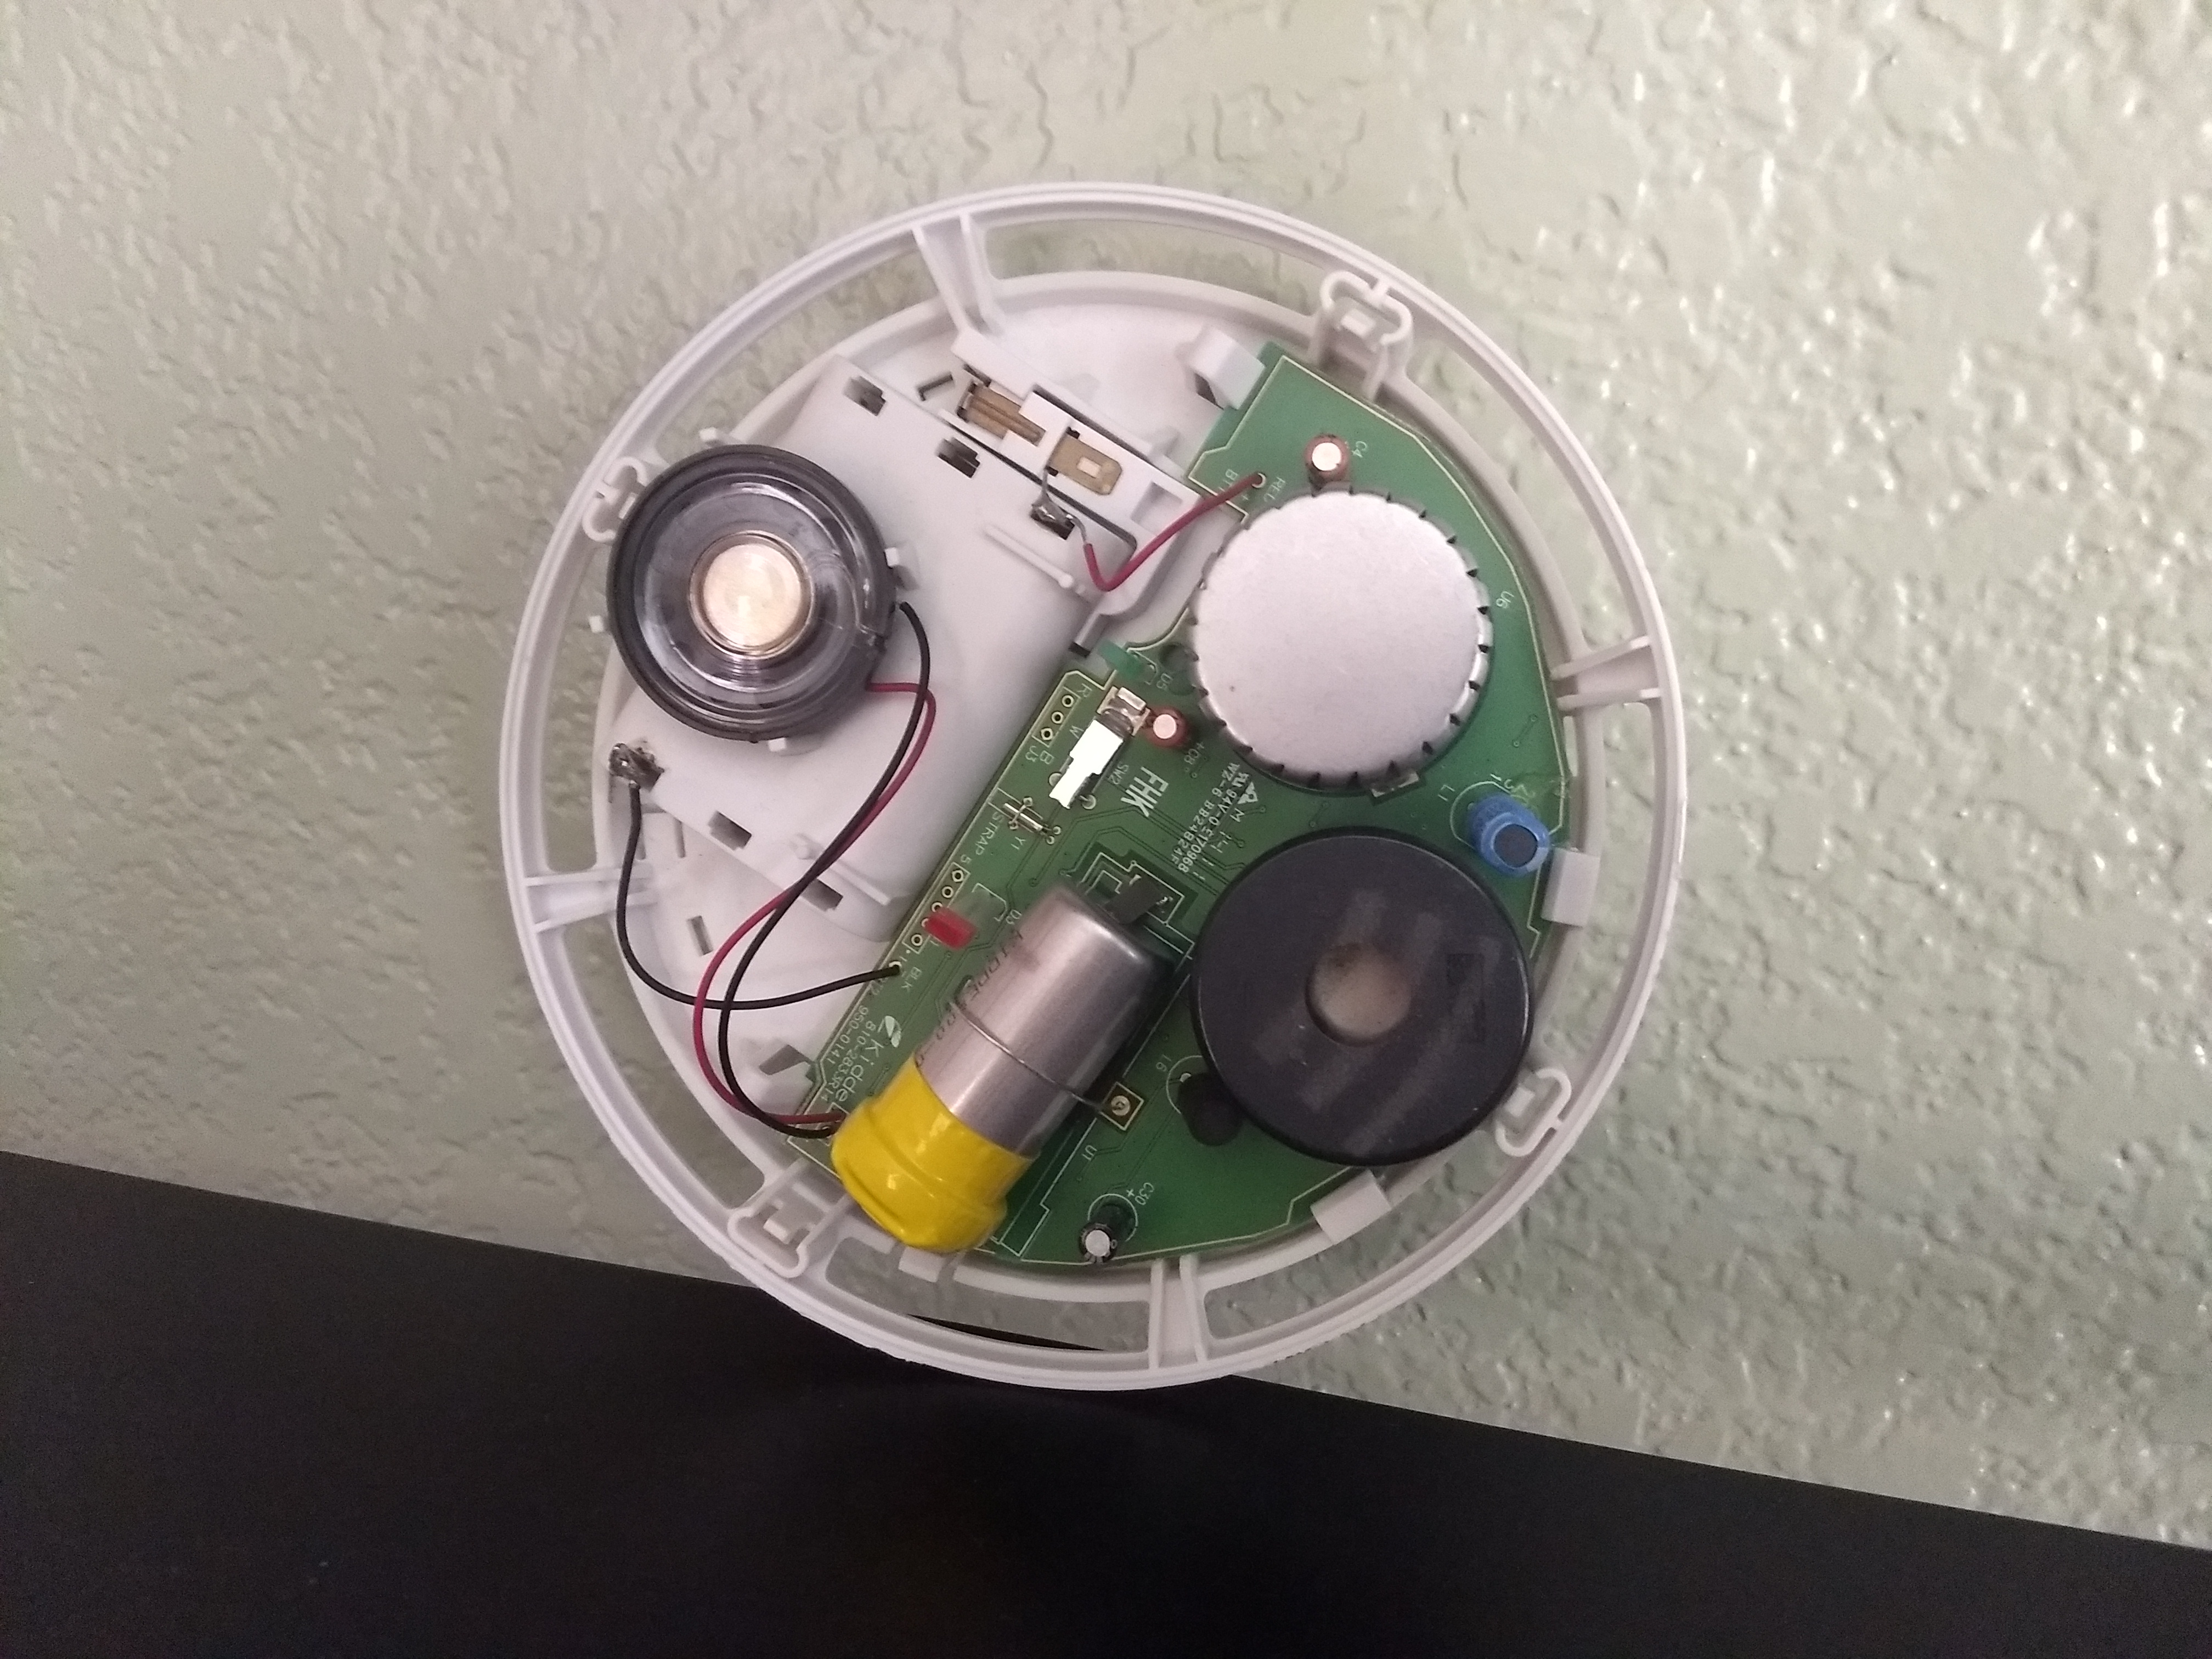
\includegraphics{./sd.jpg}
\caption{Pure Evil}
\end{figure}


    % Add a bibliography block to the postdoc
    
    
    
    \end{document}
